%%%%%
%%%%% File name  : hw4_report.tex
%%%%% Author     : Yueh-Chou Lee
%%%%% Date       : April 31, 2020
%%%%%
%%
%%%
\documentclass[a4paper,11pt]{article}
\usepackage[top=2cm,bottom=2cm,outer=2cm,inner=2cm]{geometry}
\usepackage[utf8]{inputenc}
\usepackage[T1]{fontenc}
\usepackage{fontspec}
\usepackage{xeCJK}
\usepackage{amsfonts}
\usepackage{amsmath}
\usepackage{graphicx}
\usepackage{subfigure}
\usepackage{setspace}
\usepackage[explicit]{titlesec}
\usepackage{titlesec}
\usepackage{bibentry}
\usepackage[nottoc,numbib]{tocbibind} 
\usepackage{filecontents}
\usepackage{color}
\renewcommand{\baselinestretch}{2}
\setCJKmainfont{標楷體}


\title{Machine Learning Homework 4 Report}
\author{R06221012\hspace{0.2cm}數學所\hspace{0.2cm}李岳洲}
\date{April 31, 2020}

\begin{document}

\maketitle

\begin{enumerate}
	\item \textit{\textbf{請說明你實作的 RNN 的模型架構、word embedding 方法、訓練過程 (learning curve) 和準確率為何?}}

	\begin{enumerate}

		\item Model structure:

			LSTM(

			\quad (embedding): Embedding(31889, 50)

			\quad (lstm): LSTM(embedding\_dim=50, hidden\_layers=256, num\_layers=4, batch\_first=True)

			\quad (classifier): Sequential(

			\quad \quad (0): Dropout(p=0.2, inplace=False)

			\quad \quad (1): Linear(in\_features=256, out\_features=1, bias=True)

			))\\

		\item Word embedding:

			Use the package function \textbf{\textit{gensim.models.Word2Vec}} to transform all words to vectors, then make the embedding matrix by using those all vectors.\\

\newpage

		\item Learning curve figure:\\

		\begin{figure}[htp]
		    \begin{center}
		    		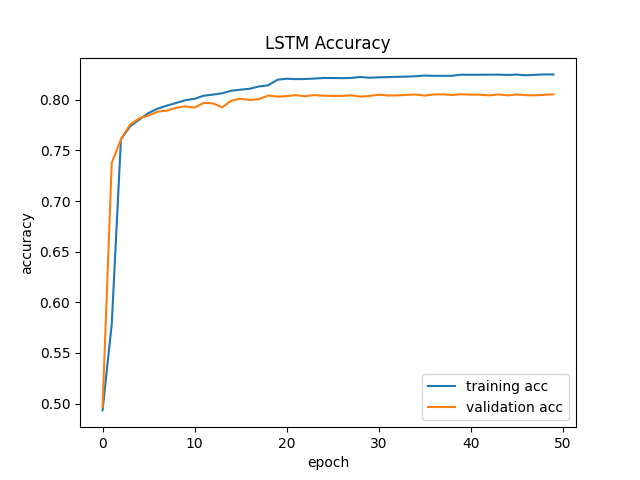
\includegraphics[scale=0.75]{./LSTM_acc.png}
		    	\caption{Accuracy curve}
		    \end{center}
		\end{figure}
	\end{enumerate}

	\item \textit{\textbf{請比較 BOW + DNN 與 RNN 兩種不同 model 對於 "today is a good day, but it is hot" 與 "today is hot, but it is a good day" 這兩句的分數 (過 softmax 後的數值),並討論造成差異的原因。}}\\

	\begin{enumerate}

		\item 
			\begin{table}[htp]
				\begin{center}
					\begin{tabular}{ | c | c | c |}
					  	\hline
				  		& today is a good day, but it is hot & today is hot, but it is a good day\\[0.5ex] 
				  		\hline \hline
				  		GRU & $0.607247$ & $0.976884$ \\[0.2ex]
				  		\hline
				  		BOW + DNN & $0.766139$ & $0.766139$ \\[0.2ex]
				  		\hline
					\end{tabular}
					\caption{Results}
				\end{center}
			\end{table}

		\item Discussion:

			The probabilities of two sentences are different in GRU model and are the same in BOW + DNN model. Because BOW does only collect all words into the bag but disregarding grammar and even word order.

	\end{enumerate}

\newpage
	
	\item \textit{\textbf{請敘述你如何 improve performance(preprocess、embedding、架構等等),並解釋為何這些做法可以使模型進步,並列出準確率與 improve 前的差異。}}

	\begin{enumerate}
		\item Model structure:

			GRUSentiment(

  			\quad (embedding): Embedding(31889, 50)
  
  			\quad (gru): GRU(embedding\_dim=50, hidden\_layers=512, num\_layers=6, batch\_first=True, dropout=0.2)

  			\quad (classifier): Sequential(

    		\quad \quad (0): Linear(in\_features=512, out\_features=1, bias=True)

    		))\\

    	\item Word embedding:

    		Use the package function \textbf{\textit{gensim.models.Word2Vec}} to transform all words to vectors, then make the embedding matrix by using those all vectors.\\

		\item Results:\\

			\begin{table}[htp]
				\begin{center}
					\begin{tabular}{ | c | c | c | c | c | c |}
					  	\hline
				  		& Training accuracy & Training loss & Validation accuracy & Validation loss & Test accuracy\\[0.5ex] 
				  		\hline \hline
				  		LSTM & $0.825083$ & -- & $0.800862$ & -- & --\\[0.2ex]
				  		\hline
				  		GRU & $0.842060$ & $0.363514$ & $0.821499$ & $0.406715$ & $0.82528$\\[0.2ex]
				  		\hline
					\end{tabular}
					\caption{Comparison table}
				\end{center}
			\end{table}

		\item Discussion:

			GRU forgets as well as input gates. GRU uses less training parameters and therefore use less memory, execute faster and train faster than LSTM, however, LSTM is more accurate on the dataset using longer sequence. For our dataset, there are collected many short sentences from Twitter, therefore, using GRU will be easier to adjust parameters to get better performance. In short, if the sequence is large or accuracy is very critical, please go for LSTM whereas for less memory consumption and the faster operation go for GRU.\\

	\end{enumerate}

	\item \textit{\textbf{請描述你的semi-supervised方法是如何標記label,並比較有無semi-supervised training對準確率的影響並試著探討原因。}}

	\begin{enumerate}

		\item Methodology:

			\begin{enumerate}
				\item We train three different GRU models and use them to predict the non-label training dataset.

				\item Ensemble those three results to label the non-label training dataset, if there is a sentence marked as 1 more than twice, then this sentence will be labeled 1.

				\item Combine this new labeled dataset with the original training dataset, then train the GRU model again.\\
			\end{enumerate}

		\item Results:\\

			\begin{table}[htp]
				\begin{center}
					\begin{tabular}{ | c | c | c | c | c | c |}
					  	\hline
				  		& Training acc & Training loss & Validation acc & Validation loss & Test acc\\[0.5ex] 
				  		\hline \hline
				  		LSTM & $0.825083$ & -- & $0.800862$ & -- & --\\[0.2ex]
				  		\hline
				  		GRU & $0.842060$ & $0.363514$ & $0.821499$ & $0.406715$ & $0.82327$\\[0.2ex]
				  		\hline
				  		GRU (semi-supervised) & $0.897974$ & -- & $0.835606$ & -- & $0.82815$ \\[0.2ex]
				  		\hline
					\end{tabular}
					\caption{Comparison table}
				\end{center}
			\end{table}

		\item Discussion:\\

	\end{enumerate}

\end{enumerate}
\end{document}